\documentclass[UTF8,a4paper,notitlepage]{ctexart}%中括号里按需设置
%标题与标题页设置
\usepackage[all,pdf]{xy}%用于绘图
\usepackage{amsmath}%用于公式中输入汉字
\usepackage{amssymb}%大写空心R
\usepackage{mathtools}%排版多行公式
\usepackage{graphicx}%插入图片
%\usepackage{tickz}%绘图支持
%\usepackage{shadow}%阴影支持
\usepackage{listings}%用于排版代码
\usepackage{ntheorem}
\usepackage{booktabs}%用于三线表
%\theoremstyle{nonumberplain}
\newtheorem{definition}{定义}
\newtheorem{lemma}{引理}[section]
\newtheorem{thm}{定理}[section]
\newtheorem{remark}{注}
\theoremstyle{nonumberplain}
\newtheorem{proof}{证明}%定理有号,证明无号
%以上三行用于无编号定义(理)
%页眉页脚设置
\usepackage{fancyhdr}
\pagestyle{fancy}%使用fancy风格,即6型
\fancyhf{}%清除所有页眉页脚
\cfoot{\thepage}%页脚居中页码
\lhead{数学科普日}
\rhead{中国科学院大学}
\usepackage{tabularx}
\usepackage{diagbox}%用于“课程表型”
\begin{document}
\ctexset{
        section={
            format+=\zihao{4}\songti\raggedright,
            name={第,部分},
            number=\arabic{section},
        }
    }
$$\textbf{\songti\zihao{3} 泊松方程的蒙特卡洛算法}$$
\begin{center}
    \text{\fangsong\zihao{4} 计算数学所 \quad 刘乐}    
\end{center}

\begin{center}
    \textbf{\zihao{5} 序 \quad 言}
\end{center}
\par
首先,感谢的是数学院研究生会组织的这次数学科普活动,
为我们不同研究方向的同学提供了一个交流的平台.\par
在这篇文章中,我分享的内容是求解泊松方程的蒙特卡洛算法.
目前,求解偏微分方程的主流方法包括有限差分法、有限元方法及
有限体积法等.这些均是确定性算法,相对于它们,蒙特卡洛算法
是一种随机算法.它基于的是概率论中的大数定律,将方程的解在某点
处的值转化为某一个随机变量的期望,然后用独立采样的平均值去逼近这个期望,
以达到近似方程解的效果.\par 
蒙特卡洛算法求解泊松方程的好处主要体现在两个方面.一是,它
相较于其他算法,十分便于并行化,从而有利于计算速度的提高;二是,
它的结论特别直观,可以独立求出微分方程的解在任意一点处的函数值.这两点好处
将在文中呈现.\par 
已有的结论是关于调和方程的情形,我们对一般情形的泊松方程
的蒙特卡洛算法进行了探究,给出了相应的结论,并通过数值算例
来展示算法的计算效果.\par 
下面分享给大家.
\zihao{-4}
\fangsong
\section{问题描述}
泊松方程$-\Delta u=f$是椭圆型方程
的代表,特别地,当$f\equiv 0$
时,称为调和方程.\par
在静电学中很容易遇到泊松方程,如:$-\Delta \Phi =\frac{\rho }{\epsilon _0} $,
这里$\Phi$表示电势,$\rho$是电荷体密度,$\epsilon _0$
是真空电容率.如果空间中某区域静带电粒子为0,则$\rho=0$,
此时就变为了调和方程$-\Delta \Phi =0$.\par
本文考虑二维泊松方程的Dirichlet边值问题:
\begin{equation}
    \begin{cases}
    -\Delta u(x,y)=f(x,y),(x,y)\in \varOmega ,\\
    u(x,y)=\varphi (x,y),(x,y)\in\partial \varOmega ,
    \end{cases}
\end{equation}
这里$\Omega$是求解区域,$\partial \Omega$是$\Omega$的边界.
\section{数值方法}
简单起见,考虑正方形区域$\varOmega=[a,b]\times [a,b]$.
\subsection{先睹为快}
我们以调和方程为例,先看看结论.
比如,我们要求取图1中红色标记点$(x,y)$(或$(i,j)$)处方程(1)的解$u(x,y)$(或$u_{i,j}$)的近似值.
\begin{figure}[ht]%浮动体
    \centering
    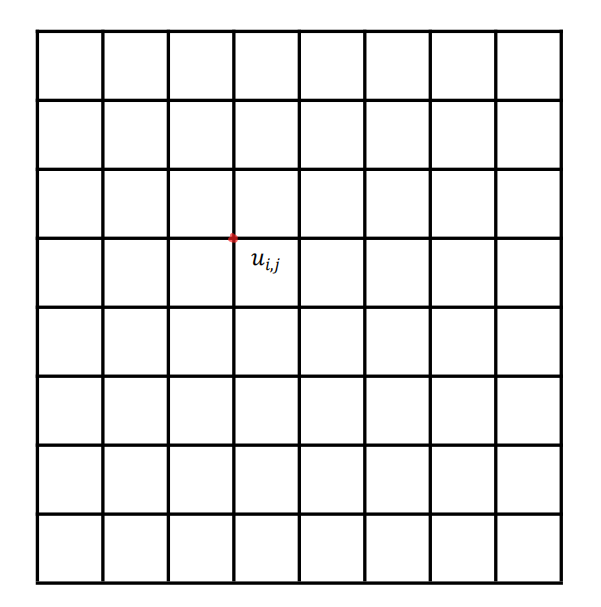
\includegraphics[scale=0.5]{tp2.png}
\caption{随机游走1}\label{fig:tp2}
\end{figure}\par
这可以通过等概率的随机游走来完成.具体地,从网格点$(x,y)$ 
处出发,沿着网格线朝着四个方向均以$\frac{1}{4}$的概率随机游走,当走到区域的边界$(x^{(1)},y^{(1)})$时,则停止,
并记下此时边界处的函数值$\varphi(x^{(1)},y^{(1)})$,这是第一次实验;就像这样,
反复独立地做$N$(充分大)次实验,可以得到序列
$\{\varphi(x^{(k)},y^{(k)})\}_{k=1}^{N}$,
那么
\begin{equation*}
    \frac{1}{N}\sum_{k = 1}^{N} \varphi(x^{(k)},y^{(k)})\stackrel{p,\varepsilon }{\approx}u(x,y) ,
\end{equation*}
这里$\stackrel{p,\varepsilon}{\approx }$表示以概率$p$落在区间
$[u(x,y)-\varepsilon ,u(x,y)+\varepsilon ]$内.可以证明(见后文),
对于任意的$\varepsilon >0$,
当$N$充分大且网格剖分足够细时,$p$都能趋于1.

\subsection{五点差分格式回顾}
将$[a,b]$剖分成$n$份,设步长为$h=\frac{b-a}{n} $,
设格点横纵坐标$x_i=y_i=a+ih,0\leq i\leq n $.\par
当$1\leq i,j\leq n-1 $时,由
\begin{gather}%罗列多个公式
    \frac{\partial ^2 u}{\partial  x^2}(x_i,y_i)\approx 
    \frac{1}{h^2}[u(x_{i-1},y_j)-2u(x_i,y_j)+u(x_{i+1},y_j)], \nonumber\\
    \frac{\partial ^2 u}{\partial  y^2}(x_i,y_i)\approx 
    \frac{1}{h^2}[u(x_{i},y_{j-1})-2u(x_i,y_j)+u(x_{i},y_{j+1})],\nonumber
\end{gather}
将它们代入微分方程$(1)$,并用$u_{i,j}$代替$u(x_i,y_j)$可得五点差分格式:
\begin{gather}%罗列多个公式
    u_{i,j}=\frac{1}{4}[u_{i,j-1}+u_{i-1,j}+u_{i+1,j}+u_{i,j+1}]
    +\frac{1}{4}h^2f(x_i,y_j), \\
    u_{0,j}=\varphi (a,y_j),u_{n,j}=\varphi (b,y_j),\\
    u_{i,0}=\varphi (x_i,a),u_{i,n}=\varphi (x_i,b),
\end{gather}
这里$1\leq i,j\leq n-1$.
\subsection{辛钦大数定律回顾}
\begin{lemma}
    设$\{X_k\}_{k=1}^{\infty}$为独立同分布
    随机变量序列,若$E[X_1]=\mu $存在,
    则 $\frac{1}{N}\sum_{k = 1}^{N}X_k$依概率收敛于
    $\mu$,
    即对任意的$\varepsilon >0$都有
    \begin{equation*}
      \lim_{N \to \infty}  P\left\{\left\lvert \frac{1}{N}\sum_{k= 1}^{N} X_k -\mu\right\rvert<\varepsilon  \right\} =1  .  
    \end{equation*}    
\end{lemma}
\subsection{主要思想}
对于$u_{i,j},1\leq i,j\leq n-1$,如果我们能找到一个随机变量$X_{i,j}$,
使得$u_{i,j}=E[X_{i,j}]$,那么由辛钦大数定律,
取$X_k=X_{i,j},\forall k$,则$\frac{1}{N}\sum_{k = 1}^{N}X_n$依概率收敛于
$u_{i,j}$,那么我们对随机变量$X_{i,j}$
独立采样$N$(充分大)次,再求平均值,即可作为$u_{i,j}$
的近似值.\par
所以关键在于寻找满足要求$E[X_{i,j}]=u_{i,j}$的随机变量$X_{i,j}$.

\subsection{先猜后证}
\subsubsection{调和方程的情形}
\subsubsection*{猜想}
考虑最简单的调和方程,只有一个未知格点值的情况,如图2:
\begin{figure}[ht]%浮动体
    \centering
    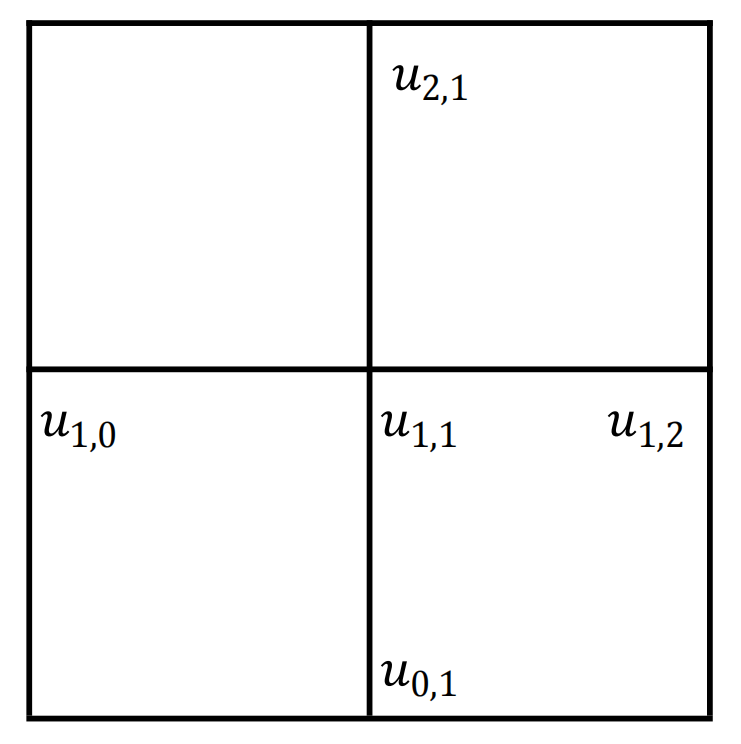
\includegraphics[scale=0.3]{tp1.png}
\caption{随机游走2}\label{fig:tp1}
\end{figure}\\
由方程(2)可知
$u_{1,1}=\frac{1}{4}[u_{1,0}+u_{0,1}+u_{2,1}+u_{1,2}]$,
显然,它是离散型随机变量
\begin{equation*}
    X_{1,1}\sim \binom{u_{2,1}\quad u_{1,0}\quad u_{0,1}\quad u_{1,2}}{1/4 \quad 1/4 \quad 1/4 \quad 1/4 } 
\end{equation*}
的期望.而随机变量$X_{1,1}$可以看成从网格坐标$(1,1)$
出发,沿着网格线朝着四个方向均以$\frac{1}{4}$的概率随机游走,
每步走一格,走到边界点则停止,停止时,
该边界点处的函数值.\par
下面内容将基于这种思想进行推广,并给出证明.
\subsubsection*{推广与证明}
\begin{definition}
    设一族随机变量$\{X_{i,j},1\leq i,j\leq n-1\}$,其中
$X_{i,j}$表示从网格坐标$(i,j)$处沿着网格线朝着四个方向均以$\frac{1}{4}$的概率随机游走,
每步走一格,走到边界点则停止,停止时,
该边界点处的函数值.
\end{definition}
\begin{thm}
    $E[X_{i,j}]=u_{i,j},\forall 1\leq i,j \leq n-1.$
\end{thm}
\begin{proof}
    设$\varphi _{s,t}$表示边界网格点$(s,t)$处的函数值,
    又随机变量$V$表示第一步随机游走的方向,
    它的取值为$0,1,2,3$,分别代表上、下、左、右.
    则由条件概率公式,有
\begin{equation}
    \begin{split}
        &P(X_{i,j}=\varphi _{s,t})\\
        &=P(V=0)P(X_{i,j}=\varphi _{s,t}|V=0)
         + P(V=1)P(X_{i,j}=\varphi _{s,t}|V=1)\\
         &+ P(V=2)P(X_{i,j}=\varphi _{s,t}|V=2)
    + P(V=3)P(X_{i,j}=\varphi _{s,t}|V=3) \\
    &=\frac{1}{4}[P(X_{i+1,j}=\varphi _{s,t})
         + P(X_{i-1,j}=\varphi _{s,t})\\
         &+ P(X_{i,j-1}=\varphi _{s,t})
    + P(X_{i,j+1}=\varphi _{s,t}) ],
    \nonumber
    \end{split} 
\end{equation} 
两边同时乘以$\varphi _{s,t}$,有:
\begin{equation}
    \begin{split}
        \varphi _{s,t}P(X_{i,j}=\varphi _{s,t})
        &=\frac{1}{4}\varphi _{s,t}[P(X_{i,j-1}=\varphi _{s,t})
         + P(X_{i,j+1}=\varphi _{s,t})\\
         &+ P(X_{i-1,j}=\varphi _{s,t})
    + P(X_{i,j}=\varphi _{s,t})],\nonumber
    \end{split} 
\end{equation}\\
两边关于$(s,t)$求和即得:
\begin{equation}
    E[X_{i,j}]=\frac{1}{4}(
        E[X_{i,j-1}]+E[X_{i,j+1}]+
        E[X_{i-1,j}]+E[X_{i+1,j}]).\nonumber
\end{equation}
此即为五点差分格式所满足的方程,由五点差分格式线性方程组
解的存在唯一性可得:
$E[X_{i,j}]=u_{i,j},\forall 1\leq i,j \leq n-1.$
\end{proof} 
\subsubsection{一般泊松方程的情形}
\subsubsection*{猜想}
为了构造相关随机变量,我们先考虑$n=3$的情形,如图3所示:
\begin{figure}[ht]%浮动体
    \centering
    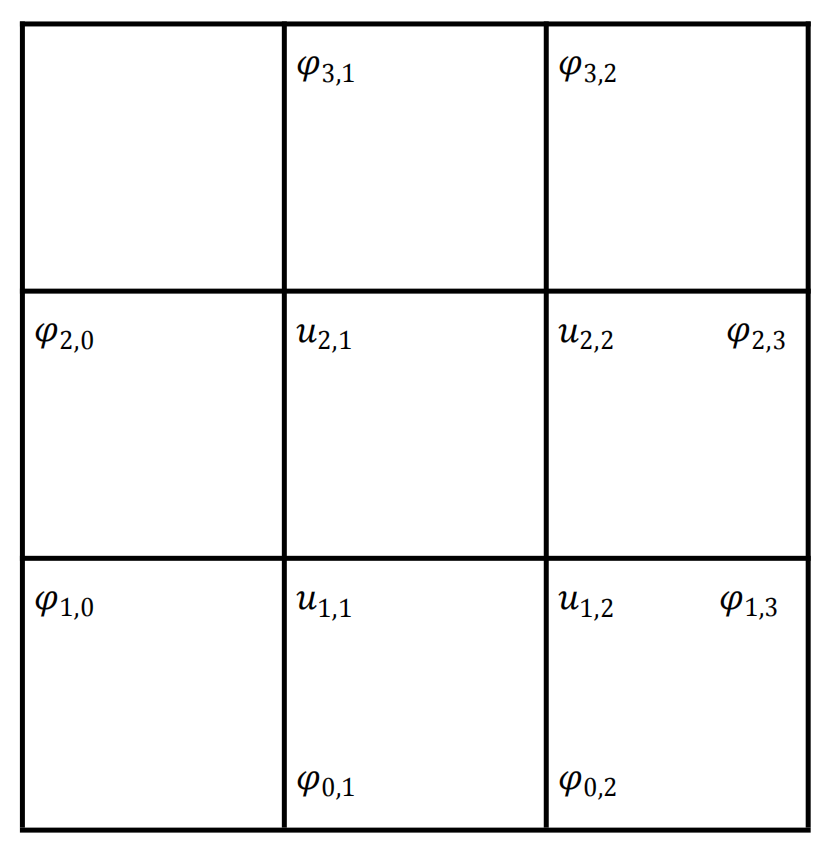
\includegraphics[scale=0.3]{tp3.png}
\caption{n=3的情况}\label{fig:tp3}
\end{figure}\\
直接求解方程(2)系数矩阵的逆矩阵,可得关系
\begin{equation}
    \begin{bmatrix}
        u_{1,1}\\
        u_{1,2}\\
        u_{2,2}\\
        u_{2,1}
    \end{bmatrix}
=\begin{bmatrix}
    7/24 & 1/12 & 1/24 & 1/12\\
    1/12 & 7/24 & 1/12 & 1/24\\
    1/24 & 1/12 & 7/24 & 1/12\\
    1/12 & 1/24 & 1/12 & 7/24
\end{bmatrix}
\left(
    \begin{bmatrix}
        \varphi _{1,0}+\varphi _{0,1}\\
        \varphi _{0,2}+\varphi _{1,3}\\
        \varphi _{3,2}+\varphi _{2,3}\\
        \varphi _{3,1}+\varphi _{2,0}
    \end{bmatrix}
    +
    \begin{bmatrix}
        h^2f_{1,1}\\
                h^2f_{1,2}\\
                h^2f_{2,2}\\
                h^2f_{2,1}
    \end{bmatrix}
\right) ,\nonumber
\end{equation}
此系数矩阵乘以2,即为概率矩阵.
再结合五点差分格式
\begin{equation}
    u_{i,j}=\frac{1}{4}[u_{i,j-1}+u_{i-1,j}+u_{i+1,j}+u_{i,j+1}]
    +\frac{1}{4}h^2f(x_i,y_j)\nonumber
\end{equation}
知一点电势受它周围四点影响,同时受本点电荷密度的影响,
那么由递推关系,亦受周围四点电荷密度的影响,扩散出去
,进而受所有点的电荷密度的影响,那么影响程度是怎么样的
呢?
由上面$n=3$的式子情况,比如$u_{1,1}$受内部电荷影响的量为
\begin{equation}
    \frac{1}{4}\left(
        \frac{7}{6}h^2f_{1,1}+
        \frac{1}{3}h^2f_{1,2}+
        \frac{1}{6}h^2f_{2,2}+
        \frac{1}{3}h^2f_{2,1}
    \right) ,
\nonumber
\end{equation}
由前面的系数的大小,我们就猜想应该和随机游走
经过的次数有关.随机游走时,经过内网格点$(k,l)$一次加一次$\frac{1}{4}h^2f_{k,l}$.
这里系数不是整数,它体现的是次数的期望,我们下面需要对这个猜想进行证明.\\
\subsubsection*{推广与证明}
\begin{definition}
设随机变量$O_{i,j}^{k,l}$表示从任意网格坐标$(i,j)$出发
沿着网格线朝着四个方向均以$\frac{1}{4}$的概率随机游走,
每步走一格,到边界则停止,到停止时,经过内网格坐标$(k,l)$的次数.
这里,当$(i,j)$为边界网格坐标时,
$O_{i,j}^{k,l}\equiv 0$.
\end{definition}
\begin{definition}
设电势积累随机变量为
\begin{equation}
    C_{i,j}=\sum\limits_{k,l}\left(\frac{1}{4}h^2f_{k,l}\right)O_{i,j}^{k,l} .\nonumber
\end{equation}
\end{definition}
\begin{thm}
    对于任意的内网格坐标$(i,j)$,下式成立:
    \begin{equation}
        E[C_{i,j}]=
\frac{1}{4}
(E[C_{i,j-1}]+E[C_{i-1,j}]+
E[C_{i+1,j}]+E[C_{i,j+1}])+\frac{1}{4}h^2f_{i,j} .\nonumber
    \end{equation}
\end{thm}
\begin{proof}
    记
    \begin{equation}
        \delta_{(i,j),(k,l)}=\begin{cases}
            1,&(i,j)=(k,l)\\
            0,&(i,j)\neq (k,l)\nonumber
        \end{cases},
    \end{equation}
    由
    \begin{equation}
        E[O_{i,j}^{k,l}]=\delta_{(i,j),(k,l)}
        +\frac{1}{4}
        (E[O_{i,j-1}^{k,l}]+E[O_{i-1,j}^{k,l}]+
        E[O_{i+1,j}^{k,l}]+E[O_{i,j+1}^{k,l}])\nonumber
    \end{equation}
两边同乘以$\frac{1}{4}h^2f_{k,l}$,可得
\begin{equation}
    \begin{split}
        \frac{1}{4}h^2f_{k,l}E[O_{i,j}^{k,l}]
        &=\frac{1}{4}h^2\delta_{(i,j),(k,l)}f_{k,l}
        +\frac{1}{4}\times\frac{1}{4}h^2f_{k,l}
        (E[O_{i,j-1}^{k,l}]+E[O_{i-1,j}^{k,l}]\\
        &+E[O_{i+1,j}^{k,l}]+E[O_{i,j+1}^{k,l}]),\nonumber
    \end{split}
\end{equation}
关于$(k,l)$求和,并由期望的线性性质即得
\begin{equation}
        E[C_{i,j}]=
\frac{1}{4}
(E[C_{i,j-1}]+E[C_{i-1,j}]+
E[C_{i+1,j}]+E[C_{i,j+1}])+\frac{1}{4}h^2f_{i,j} .\nonumber 
\end{equation}
\end{proof}
\begin{definition}
    对于任意网格坐标$(i,j)$,记
    随机变量$Y_{i,j}=X_{i,j}+C_{i,j}$,
    即其表示从任意网格坐标$(i,j)$出发
    沿着网格线朝着四个方向均以$\frac{1}{4}$的概率随机游走,
    每步走一格,
    到边界则停止,到停止时,
    经过内网格坐标的电势的积累与到达的
    边界网格坐标处的电势之和.
\end{definition}
\begin{thm}
    对于任意的网格坐标$(i,j)$,成立
    \begin{equation}
E[Y_{i,j}]=u_{i,j}.\nonumber
    \end{equation}
\end{thm}
\begin{proof}
当$(i,j)$为边界网格坐标时,由
$E[C_{i,j}]=0,E[X_{i,j}]=\varphi _{i,j}=u_{i,j}$
知$E[Y_{i,j}]=u_{i,j}$;\\
当$(i,j)$是内网格坐标时,
\begin{gather}
    E[X_{i,j}]=\frac{1}{4}(
        E[X_{i,j-1}]+E[X_{i,j+1}]+
        E[X_{i-1,j}]+E[X_{i+1,j}]),\nonumber\\
        E[C_{i,j}]=\frac{1}{4}
        (E[C_{i,j-1}]+E[C_{i-1,j}]+
        E[C_{i+1,j}]+E[C_{i,j+1}])+\frac{1}{4}h^2f_{i,j} ,\nonumber 
\end{gather}
相加,即得
\begin{equation}
    E[Y_{i,j}]=
\frac{1}{4}
(E[Y_{i,j-1}]+E[Y_{i-1,j}]+
E[Y_{i+1,j}]+E[Y_{i,j+1}])+\frac{1}{4}h^2f_{i,j} ,\nonumber 
\end{equation}
知$E[Y_{i,j}]$与泊松方程五点差分格式
满足相同的线性方程组,由解的唯一性,
可得$E[Y_{i,j}]=u_{i,j}.$
\end{proof}
\subsection{算法设计}
有了函数值$u_{i,j}$的近似为随机变量$Y_{i,j}$的期望,
则由辛钦大数定律,
对于任意给定的$\varepsilon>0$, 
$\frac{1}{N}\sum_{k = 1}^{N}y_{i,j}^{(k)} \in\left[ u_{i,j}-\varepsilon ,u_{i,j}+\varepsilon \right] $  
以概率$p(N,\varepsilon)$成立,且$\lim_{N \to \infty}p(N,\varepsilon)=1$.
其中$\left\{y_{i,j}^{(k)}\right\}_{k=1}^{N} $为$Y_{i,j}$的$N$
次独立采样.\\
根据我们的理论可以给出以下算法:\\
\\
\begin{tabular*}{\textwidth}{l}
\toprule
$$\textbf{\songti 算法}$$泊松方程的蒙特卡洛算法\\
\midrule
1.$$\textbf{\songti 输入}$$:区域$[a,b]\times [a,b]$边长剖分的个数$n$,要求函数值的网格\\
坐标$(i,j)$,采样次数$N$.\\
2.$$\textbf{\songti 初始化}$$:内电势积累$C=0$,边界电势积累$X=0$,步长$h=\frac{b-a}{n}$,\\
记录采样次数的变量$k=0$,当前网格坐标$(ii,jj)=(i,j)$,当前实际\\
坐标$(x_{ii},y_{jj})=(a+ih,a+jh)$,随机变量的值$r$,网格坐标$(i,j)$处\\
函数值的近似$rs=0$.\\
3.$$\textbf{\songti 过程}$$:\\
4.
$$\textbf{for}$$ $k=1,2,\dots,N$ $$\textbf{do}$$\\
5.
$$\textbf{while}$$ $(ii,jj)$是内网格坐标 $$\textbf{do}$$\\
6.
得到实际坐标$(x_{ii},y_{jj})=(a+iih,a+jjh)$.\\
7.
更新$C=C+\frac{1}{4}h^2f(x_{ii},y_{jj})$.\\
8.
从$\left\{0,1,2,3\right\} $中等概率采样,得到随机变量的值$r$.\\
9.
$$\textbf{if}$$(r=0)
ii=ii+1;\\
10.$$\textbf{elif}$$(r=1)
ii=ii-1;\\
11.$$\textbf{elif}$$(r=2)
jj=jj-1;\\
12.$$\textbf{else}$$
jj=jj+1;\\
13.$$\textbf{end}$$
$$\textbf{if}$$\\
14.$$\textbf{end}$$
$$\textbf{while}$$\\
15.
得到实际坐标$(x_{ii},y_{jj})=(a+iih,a+jjh)$.\\
16.
更新$X=X+\varphi (x_{ii},y_{jj})$.\\
17.
还原坐标$(ii,jj)=(i,j)$.\\
18.
$$\textbf{end}$$
$$\textbf{for}$$\\
19.输出:网格坐标$(i,j)$处函数值的近似$rs=\frac{X+C}{N}$.\\
\bottomrule
\end{tabular*}


\section{收敛性分析与数值算例}
\subsection{收敛性分析}
设$\omega $是内网格坐标集合,对于五点差分格式
有结论:
\begin{lemma}
    \begin{equation*}
        max_{(i,j)\in \omega}\left\lvert u(x_i,y_j)-u_{i,j}\right\rvert 
    \leq C(\Omega,f,\varphi )h^2,
    \end{equation*}
这里$C(\Omega,f,\varphi )$是依赖于$\Omega,f,\varphi$的正常数.
\end{lemma}
由前面知,对于任意给定的$\varepsilon>0$, 
\begin{equation*}
    \frac{1}{N}\sum_{k = 1}^{N}y_{i,j}^{(k)} \in\left[ u_{i,j}-\frac{1}{2}\varepsilon ,u_{i,j}+\frac{1}{2}\varepsilon \right] 
\end{equation*}
以概率$p(N,\frac{1}{2}\varepsilon)$成立,且$\lim_{N \to \infty}p(N,\frac{1}{2}\varepsilon)=1$.
其中$\left\{y_{i,j}^{(k)}\right\}_{k=1}^{N} $为$Y_{i,j}$的$N$
次独立采样.\\
由引理$3.1$,当$n$充分大时,有
\begin{equation*}
    \left[ u_{i,j}-\frac{1}{2}\varepsilon ,u_{i,j}+\frac{1}{2}\varepsilon \right] \subset
    \left[ u(x_i,y_j)-\varepsilon ,u(x_i,y_j)+\varepsilon \right] ,
\end{equation*}
所以 
\begin{equation*}
    \frac{1}{N}\sum_{k = 1}^{N}y_{i,j}^{(k)} \in \left[ u(x_i,y_j)-\varepsilon ,u(x_i,y_j)+\varepsilon \right] 
\end{equation*}
以概率$q(N,\varepsilon)>p(N,\frac{1}{2}\varepsilon)$成立,更有$\lim_{N \to \infty}q(N,\varepsilon)=1$.
\subsection{数值算例}
考虑算例:
\begin{equation}
    \begin{cases}
    -\Delta u(x,y)=(\pi^2-1)e^x\sin(\pi y),(x,y)\in(0,1)\times (0,1), \\
    u(0,y)=\sin(\pi y),u(1,y)=e\sin(\pi y),y\in[0,1],\\
    u(x,0)=0,u(x,1)=0,x\in(0,1),\nonumber
    \end{cases}
\end{equation}
该问题的精确解为$u(x,y)=e^x\sin(\pi y)$.\\
我们对每个内网格点$(i,j)$均利用上面蒙特卡洛算法求解,得到 
相应的近似值为$rs_{i,j}$,
然后看平均误差$merror$的大小,这里我们采用$1-$范数,
即
\begin{equation*}
    merror=\frac{1}{n^2}\sum_{i= 1}^{n}\sum_{j= 1}^{n}\left\lvert rs_{i,j}-u(x_i,y_j)\right\rvert  .   
\end{equation*}
\\
计算结果如下:\\
\\
\begin{tabular}{|c|c|c|c|c|}
\hline
\diagbox{N}{merror}{n} & 10 & 20 & 40 & 80 \\
\hline
10 & 0.253955 &0.250992  &0.227093  & 0.227312  \\
\hline
100 & 0.0847661& 0.0806093& 0.0740826
&0.0720648 \\
\hline
1000 & 0.0234798& 0.0256761 &  0.0235552
&0.023018 \\
\hline
\end{tabular}
\subsection{误差定性分析}
通过表格可以看出,当区域边长剖分个数$n$固定时,
$merror$随着采样步数$N$的增加,明显变小;
当采样步数$N$固定时,$merror$随着
区域边长剖分个数$n$的增加,变化较小.\par
这是可以理解的.事实上,我们的误差来源于两部分,
一是,五点差分格式的解$u_{i,j}$与真实解$u(x_i,y_j)$
的误差;二是,蒙特卡洛算法所得结果$rs_{i,j}$与
五点差分格式的解$u_{i,j}$的误差.由引理$3.1$,
前者是二阶的,即为$O\left(1/n^2\right) $,
在本例中(区域边长为1)我们取的$n$已经足够大了,可以保证,前者带来的误差
是微乎其微了,所以主要误差在于蒙特卡洛算法,因此 
当步长增大时能够显著减少误差.
\section{总结与展望}
我们知道,用蒙特卡洛算法求每个点方程解函数值的近似
值时,求法上不依赖于周围其他点的信息,只需要采样即可,
而采样可以并行来进行,这比五点差分格式的并行处理简单得多.
另外一点好处是蒙特卡洛算法可以直接求出任意一点
处的近似值,而五点差分格式做不到这一点.特别是在高维情形,
蒙特卡洛算法几乎成了唯一的选择.\par
关于蒙特卡洛算法,本文只是粗糙地利用一下其基本原理,这个算法本身
就是一门专门而系统的学问,包括方差减小技术、重要性采样、切片抽样等等,这些 
需要将来进一步地学习.
\section{参考文献}
{\raggedright
[1]游皎,李万爱.高效蒙特卡罗方法在偏微分方程初边值问题中的应用[J].
中山大学学报:自然科学版,(2015)06-0037-05.\par
[2]刘春光.偏微分方程边值问题的蒙
特卡罗解法[D].长春:吉林大学,2004.\par
[3]Michael J.Quinn.陈文光,武永卫 等译.
MPI与OpenMP并行程序设计:C语言版[M].北京:清华大学出版社,2004.
}

\end{document}